

\begin{abstract}[\hspace*{-10pt}]
    This appendix is a postprint of the accepted work: \fullcite{van_biesbroeck_design_2025}  % Ce chapitre reprend principalement les travaux publiés dans: 
\end{abstract}

\begin{abstract}
    %Seismic fragility curves are key quantities of interest for Seismic Probabilistic Risk Assessment studies. They express the probability of failure of a mechanical structure of interest conditional to a scalar value derived from the ground motion signal coined Intensity Measure. 
%In the literature, Bayesian approaches have emerged to 
In this appendix, we propose 
an efficient modeling for the estimation of seismic fragility curves in the Bayesian context that is not based on the common probit-lognormal model. % of fragility curves.
%enable their estimation within the difficult context of limited data availability.  Yet, the probit- lognormal modeling over which most of them are based requires the use of computationally expensive {Markov chain Monte Carlo} methods for providing Bayesian estimators.  %
% In this work, we propose an efficient modeling for the estimation of fragility curves in the Bayesian context, 
We implement instead a low fidelity model of the structure's response to the ground motion signal and an objective prior. In this work, we do not limit the knowledge about the state of the structure to a  binary outcome.
The analytical expression of our modeling {allows} fast generation of estimates. Also, the representative bias arisen by the modeling choice is partly handled with a  design of experiments methodology. Finally, our approach is evaluated on a real case study. Our results prove its ability to satisfyingly overcome the irreducible bias when coupled with the design of experiments we propose. However,
they also highlight the strong limitations of such simple model, even if it takes richer information about the structural responses as inputs than only binary outcomes.
\end{abstract}


\minitoc

\section{Introduction}




The probabilistic seismic risk assessment framework (SPRA) introduced in the 1980s for the nuclear industry is based on the estimation of seismic fragility curves, for the structures and components (SCs) of interest \citep{kennedy_probabilistic_1980,kennedy_seismic_1984,park_survey_1998,kennedy_risk_1999,cornell_hazard_2004}. These curves are defined as the conditional probability that an engineering demand parameter (EDP) ---such as the interstory drift ratio--- exceeds a limit threshold, given a scalar value derived from the seismic ground motion and called intensity measure (IM). The IM can be for instance the peak ground acceleration (PGA) or a pseudo-spectral acceleration (PSA) evaluated for a given frequency and damping ratio \citep{ciano_role_2020,sainct_efficient_2020,ciano_novel_2022}. As explained in \cite{cornell_hazard_2004}, it is therefore assumed that the seismic hazard, on a given site, can be reduced to such a single indicator.


Practitioners have several data sources at their disposal to estimate fragility curves, namely: expert judgments supported by test data \citep{kennedy_probabilistic_1980,kennedy_seismic_1984,park_survey_1998,zentner_fragility_2017}, experimental data \citep{park_survey_1998,gardoni_probabilistic_2002,choe_closed-form_2007}, results of damage collected on existing structures that have been subjected to earthquakes \citep{shinozuka_statistical_2000,lallemant_statistical_2015,straub_improved_2008} as well as analytical results given by more or less refined numerical models using synthetic or real seismic excitations \citep{zentner_numerical_2010,wang_influence_2020,mandal_seismic_2016,wang_bayesian_2018,wang_seismic_2018,zhao_seismic_2020}. Over the years, many methods have been developed to estimate these curves \citep{shinozuka_statistical_2000,lallemant_statistical_2015,zentner_fragility_2017}. Nowadays, even though machine learning techniques are becoming very popular  \citep{park_rapid_2014,seo_use_2013,gidaris_kriging_2015,wang_seismic_2018,sainct_efficient_2020}, parametric fragility curves historically introduced in the SPRA framework are ubiquitous in practice and the log-normal model is the most widely used model due to its proven ability to handle limited data \citep{shinozuka_statistical_2000,lallemant_statistical_2015,straub_improved_2008,zentner_numerical_2010,wang_influence_2020,mandal_seismic_2016,hariri-ardebili_probabilistic_2016,wang_bayesian_2018,wang_seismic_2018,zhao_seismic_2020,ellingwood_earthquake_2001,kim_development_2004,mai_seismic_2017,trevlopoulos_parametric_2019,katayama_bayesian-estimation-based_2021}.

Different strategies can be implemented to estimate the parameters that define the fragility curve in the log-normal model. Among these we distinguish the Bayesian framework
%Among the different strategies that can be implemented to estimate the parameters that define the fragility curve in the log-normal model we distinguish the Bayesian framework 
\citep{gardoni_probabilistic_2002,wang_seismic_2018,katayama_bayesian-estimation-based_2021,koutsourelakis_assessing_2010,damblin_approche_2014,tadinada_structural_2017,kwag_computationally_2018,jeon_parameterized_2019,tabandeh_physics-based_2020,lee_efficient_2023}. 
This framework is interesting because it allows to solve the irregularity issues encountered %\sout{when the data availability is sparse} 
{when few data are available}. This occurs with the widely used maximum likelihood estimation coupled with a bootstrap technique to estimate a confidence interval when the data are binary, that is, when they represent the failing or non-failing state of the structure (as in the studies conducted in the \cref{part:spra} of this manuscript). In practice, binary data are encountered 
%those problems are especially encountered when resorting to complex and detailed modeling due to the calculation burden or 
when dealing with tests performed on shaking tables for instance.

In earthquake engineering, within the SPRA framework, Bayesian inference is often used to update log-normal fragility curves obtained beforehand by various approaches, by assuming independent distributions for the prior values of the parameters, such as log-normal distributions for instance \citep{tadinada_structural_2017,kwag_computationally_2018,wang_seismic_2018,katayama_bayesian-estimation-based_2021,straub_improved_2008}. In this thesis, based on the reference prior theory, we proposed the use of an objective prior, in order to remove any subjectivity that could legitimately lead to inevitable open questions on the influence of the \emph{a priori} on the quantities of interest. In all these approaches, the use of Markov chain Monte Carlo (MCMC) methods is nevertheless necessary to sample the \emph{a posteriori} distribution of the parameters, which can prove cumbersome to implement, particularly if we want a rapid first estimate of a fragility curve with limited data. 

%To circumvent this, we propose in this work an effective approach for estimating fragility curves, which avoids the use of the MCMC method, and which is based on the use of a low fidelity model to represent the structural response. Since the low-fidelity model is a linear model, we also propose an experimental design algorithm to minimize representation bias.\\

We circumvent this problem in this work by proposing an effective approach for the estimation of fragility curves, which avoids the use of the MCMC method. We rely on a low-fidelity linear model between the logarithm of the Engineering Demand Parameter and the one of the IM \citep{lallemant_statistical_2015,hariri-ardebili_probabilistic_2016,zentner_fragility_2017,ghosh_seismic_2020}. Supported by the Bayesian framework, our model benefits from a fully analytical form; that former allows an efficient implementation and a solution for fast generation of estimates with limited data. The reliability of the Bayesian scheme w.r.t.{ }its prior choice is answered as well with the derivation of an objective prior derived on the basis of the reference prior theory (see the \cref{part:ref-theory} of this manuscript). Finally, since the low-fidelity model is a linear model, we also propose a sequential planning of experiments strategy to minimize the representation bias. 
The design we suggest relies on the maximization of the information brought by the observation of a new data item onto the posterior distribution. That one is measured through global sensitivity indices described in~\cite{da_veiga_global_2015}.
%arisen from global sensitivity analysis
%that serves as measure of the information transmission by a new data item.


The remainder of this appendix is organized as follows:
the statement of our low-fidelity modeling strategy for the fragility curves estimation in a Bayesian framework is presented in \cref{lowdoe:sec:modeling}.
After a brief review devoted to global sensitivity analysis, we describe in \cref{lowdoe:sec:PE} our design for a sequential planning of experiments, taking the global sensitivity indices as a support.
\Cref{lowdoe:sec:application} is dedicated to the implementation of our methodology on a case study from the nuclear industry. Finally, \cref{lowdoe:sec:discussion} which precedes the conclusion offers a discussion on the performance of our method.
%a discussion about the performances.






\section{Low fidelity model for fragility curves}\label{lowdoe:sec:modeling}
    \subsection{Linear regression model}
    
    The fragility curve which we seek to estimate is defined by
\begin{equation}
    P_f(a) = \PP(\mathrm{EDP}>C\,|\mathrm{IM}=a).
\end{equation}
Up to a refinement of a multiplicative constant in the definition of the engineering demand parameter (EDP), $C$ can be supposed to be equal to $1$ in what follows.
The EDP is supposed to be correlated with the intensity measure (IM) as follows
\begin{equation}
    \log \mathrm{EDP} = \rho\log \mathrm{IM} + \epsilon ,
\end{equation}
where the random variable $\epsilon$ follows 
the distribution $\cN(\mu,\sigma^2)$.
Here $\rho$ is supposed unknown, as well as $\mu$ and $\sigma$. 
%Conditionally to a set of different values of the IM, the resulting values of the EDP are supposed to be independent. 




    
    \subsection{Likelihood}\label{lowdoe:sec:likelihood}

We have at our disposal a data-set composed by the tuples $(a_i,y_i)_{i=1}^k$, $a_i\in\cA\subset(0,\infty)$ denoting the measured IM from {the $i$-th seismic ground motion} signal and $y_i\in\cY\subset(0,\infty)$ denoting the structure's EDP. Conditionally to the parameter $\theta=(\rho,\mu,\sigma)$, we suppose the observations to be independent and identically distributed. As $a_i$ follows a distribution assumed to admit a density $a\mapsto h(a)$ w.r.t.{ }the Lebesgue measure and to be independent of $\theta$, the distribution of the $y_i$ is known conditionally to $(a_i,\theta)$:
    \begin{equation}
        \log y_i|a_i,\theta \sim \cN(\rho\log a_i+\mu,\sigma^2)    .
    \end{equation}
The likelihood for the parameter $\theta$ is therefore:
    \begin{equation}
        \ell_k^0(\hatmbf y,\hatmbf a|\theta) = \prod_{i=1}^k \frac{1}{\sqrt{2\pi\sigma^2}}\exp\left( -\frac{(\hat y_i-\rho\hat a_i-\mu)^2}{2\sigma^2} \right)h(a_i),
    \end{equation}
where $\hat y_i$ (resp. $\hat a_i$) denotes $\log y_i$ (resp. $\log a_i$) and $\hatmbf y$ (resp. $\hatmbf a$) denotes the vector $(\log y_i)_{i=1}^k$ (resp. $(\log a_i)_{i=1}^k$).

%for example, they are primarily introduced to separate the parameters and thus to make the posterior distribution
{
This likelihood introduces a challenge due to the lack of clear separation among the three parameters that constitute $\theta$. Within the Bayesian framework, which we develop later, this challenge could result in a posterior distribution that is hardly tractable. We address this issue by introducing the following quantities:
}
%To benefit from a likelihood that separates better the parameters and so that would make a posterior distribution more tractable later, we consider the following quantities: 
%To benefit from a more tractable likelihood, we consider the following quantities derived from the data:
    \begin{equation}
        \rho_k = \frac{\Cov_k(\hatmbf y,\hatmbf a)}{\Var_k\hatmbf a}, \quad
        \mbf z = \tilde P_{\mbf a}^{\top}(\hatmbf y - \rho_k\hatmbf a) ,
    \end{equation}
where $\Cov_k$, $\Var_k$ respectively denote the empirical covariance and variance, and the matrix $\tilde P_{\mbf a}$ is defined in \cref{lowdoe:app:sec:DiagUa}.
%{$\rho_k$ is the natural slope estimator, and $\mbf z$ is the normalized addition of the residuals and the bias.} 
Their conditional distributions are given by:
    \begin{align}
        &  \rho_k|\mbf a,\theta \sim \cN\left( \rho,\frac{\sigma^2}{k\Var_k\hatmbf a} \right), \\
        &   \mbf z | \mbf a, \theta \sim  \cN(\mu\tilde P_{\mbf a}^{\top}\mbf 1,\sigma^2D);\quad D=\diag\left(1,\dots,1,\frac{\hatmbf a^{\top}\hatmbf a}{k\Var_k\hatmbf a}\right), %\cN(\mu\mathbf{1}, \sigma^2 U_{\mbf a})
    \end{align}
where $\mbf a$ is the vector $(a_i)_{i=1}^k$, $\mbf 1$ denotes the vector of $\RR^k$ composed only of ones, and $\diag(\lambda_1,\dots,\lambda_{k-1}) $ refers to the diagonal matrix of $\RR^{(k-1)\times(k-1)}$ whose diagonal coefficients are the $(\lambda_i)_{i=1}^{k-1}$. 
%matrix $U_{\mbf a}$ is given by
% \begin{equation}
%     U_{\mbf a} = I - \frac{\hatmbf a(\frac{1}{2}\hatmbf a - \overline{\hatmbf a})^{\top}  }{k\Var_k\hatmbf a} - \frac{(\frac{1}{2}\hatmbf a - \overline{\hatmbf a}) \hatmbf a^{\top}  }{k\Var_k\hatmbf a}\ ;\quad \overline{\hatmbf a} = \frac{1}{k}\sum_{i=1}^k \log a_i.
% \end{equation}

Let us denote by $(w_i)_{i=1}^k$ the orthogonal columns of the matrix $P_{\mbf a}$ defined in \cref{lowdoe:app:sec:DiagUa}. Noticing $\rho_k = w_k^{\top}\hatmbf y$ and $\mbf z$ is spanned by the $(w_{i})_{i=1}^{k-1}$, we deduce that $\mbf z$ and $\rho_k$ are independent conditionally to $(\mbf a, \theta)$, and that the knowledge of $(\mbf z,\rho_k,\mbf a)$ is equivalent to the one of $(\mbf y,\mbf a)$ or $(\hat{\mbf y},\hat{\mbf a})$.
Thus, the likelihood issued from the observations of $(\mbf z, \rho_k, \mbf a)$ is 
\begin{equation}\label{lowdoe:eq:likelihood}
     \ell_k(\mbf z,\rho_k,\mbf a|\theta) = h(\mbf a)\frac{\|\hatmbf a-\overline{\hatmbf a}\|}{\sqrt{2\pi\hatmbf a^{\top}\hatmbf a}\sigma}\exp\left(-\frac{(z_{k-1}-\mu \sqrt{k})^2}{2\sigma^2\frac{\hatmbf a^{\top}\hatmbf a}{\|\hatmbf a-\overline{\hatmbf a}\|^2}}\right)\exp\left({-\frac{(\rho_k-\rho)^2}{2\sigma^2/(k\Var_k\hatmbf a)}}\right)\prod_{i=1}^{k-2}\frac{1}{\sqrt{2\pi}\sigma}\exp\left(-\frac{z_i^2}{2\sigma^2}\right),
\end{equation}
where $\overline{\hatmbf a} = \frac{1}{k}\sum_{i=1}^k \log a_i$, and $h(\mbf a)=\prod_{i=1}^kh(a_i)$.


    \subsection{Prior and posterior}\label{lowdoe:sec:priorposterior}
%


Within a Bayesian context, the parameter of interest $\theta$ is itself a random variable taking values in a space $\Theta\subset\RR^2\times(0,\infty)$ and following a distribution called the prior.
We take as a support the reference prior theory (see the \cref{part:ref-theory} of this manuscript) to justify the choice of the Jeffreys prior for $\theta$, derived from the likelihood expressed in \cref{lowdoe:eq:likelihood}.
Conditionally to $\mbf a$, that former is a Gaussian density, making the associated Fisher information matrix being:
       \begin{equation}    
        \cI(\theta) = \int_{\cA^k}\left(\begin{array}{ccc}
             k\frac{\|\hatmbf a - \overline{\hatmbf a}\|^2}{\sigma^2\hatmbf a^{\top}\hatmbf a}&  0&0\\
             0&k\frac{2}{\sigma^2}&0 \\
             0&0& \frac{k\Var_k\hatmbf a}{\sigma^2}
        \end{array}\right) \prod_{i=1}^kh(a_i)d a_i.
    \end{equation}
The Jeffreys' prior being defined as the one whose density $J$ w.r.t.{ }the Lebesgue measure is proportional to $\sqrt{|\cI(\theta)|}$, we obtain
\begin{equation}
    J(\theta)\propto \frac{1}{\sigma^3}.
\end{equation}

Finally, the posterior distribution of $\theta$ is given by its density, which is proportional to the product of the likelihood (from \cref{lowdoe:eq:likelihood}) with the prior:
    \begin{equation}\label{lowdoe:eq:posterior}
        p(\theta|\mbf z, \mbf a,\rho_k) \propto \frac{1}{\sigma^{k+3}} \exp\left({-\frac{\sum_{i=1}^{k-2}z_i^2}{2\sigma^2}}\right) \exp\left({-\frac{k\|\hatmbf a-\overline{\hatmbf a}\|^2}{\hatmbf a^{\top}\hatmbf a}\frac{(z_{k-1}k^{-1/2}-\mu)^2}{2\sigma^2}}\right)
            \exp\left({-\frac{(\rho_k-\rho)^2}{2\sigma^2/(k\Var_k\hatmbf a)}}\right).
    \end{equation}
We recognize the above as a product of square inverse gamma distributions. More precisely, $\sigma^{-2}$ follows a gamma distribution, and $\mu$ and $\rho$ follow independent Gaussian distributions conditionally to $\sigma$.

This posterior allows to elucidate the distribution of what expresses the fragility curve: 
\begin{equation}
    P_f(a)|\theta \sim \PP( \hat y>0|\hat a,\theta) = \Phi\left(\frac{\rho\log a+\mu}{\sigma}\right) ,
\end{equation}
with $\Phi$ being the c.d.f. of a standard Gaussian distribution.

Its distribution is known \emph{a posteriori}, given that
$\frac{\rho\log a+\mu}{\sigma}$, conditionally to $(a,\mbf a,\mbf y)$ for any $a\in\cA$, is distributed as the sum
of a variable with Gaussian distribution and the square root of a variable with Gamma distribution (both variables being independent):
\begin{align}
    &\frac{\rho\log a+\mu}{\sigma}\big| a,\mbf a,\mbf y \sim \cN\left(0,\frac{\log^2 a}{k\Var_k\hatmbf a} + \frac{\hatmbf a^{\top}\hatmbf a}{k\|\hatmbf a -\overline{\hatmbf a}\|^2} \right) + \left(\rho_k\log a + \frac{z_{k-1}}{\sqrt{k}}\right)\Gamma^{1/2}(\tilde c,\tilde d) \label{lowdoe:eq:apostcf} , \\
    &\tilde c = k/2, \qquad \tilde d = \frac{1}{2}\sum_{i=1}^{k-2}z_i^2.
\end{align}



\section{Sensitivity index for design of experiments}\label{lowdoe:sec:PE}

\subsection{A review of the global sensitivity analysis}

Global sensitivity analysis (GSA) %\sout{provides an essential scope for computer experiment based studies} \clem
{is a cornerstone of uncertainty quantification studies of computer simulators}. It aims at quantifying how the uncertainties within the observed output of a model are influenced by the uncertainties of one or several of its inputs \citep{iooss_review_2015}.
More formally, in classical GSA settings, a system outputs an observed variable $Y$, supposed to be a function of input variables $Y=\eta(X_1,\dots,X_p)$, where the input $X_i$'s are assumed to follow a known distribution and to be mutually independent. 
Since the first indices introduced by \citet{sobol_sensitivity_1993}, GSA's tools measure statistically how $Y$ is impacted by one or some of the $X_i$ \citep{da_veiga_basics_2021}.
Global sensitivity indices \citep{da_veiga_global_2015} are quantities whose class regroups a large range of these tools.
%
%Several of those measuring tools are regrouped within the class of the global sensitivity indices~\cite{DaVeiga2015}: 
According to their definition, letting $D$ be a dissimilarity measure between probability distributions, the impact of input $X_i$ onto the output $Y$ can be derived as
    \begin{equation}
        S_i = \EE_{X_i}\left[D(\PP_{Y}||\PP_{Y|X_i})\right] ,
    \end{equation}
where $\PP_Y$ is the distribution of $Y$, $\PP_{Y|X_i}$ is the conditional distribution of $Y$ given $X_i$. The choice of $D$ can depend on the expected properties. A classical example is to set $D(P||Q)=\|\EE_{X\sim P}[X]-\EE_{X\sim Q}[X]\|^2$ which gives the un-normalized Sobol' index \citep{sobol_sensitivity_1993}.



\subsection{Sequential planning of experiments via global sensitivity index maximization}

Following the idea of \citet{da_veiga_global_2015}, a judicious data acquisition strategy would be to minimize the sensitivity that the posterior would get from the observations. This way, the IM $a_{k+1}$ that has to be chosen for the next simulation which would output an EDP $y_{k+1}$, after having observed $(\mbf y, \mbf a)=(y_i,a_i)_{i=1}^k$ is the one such that the following index is maximized:
    \begin{equation}\label{lowdoe:eq:dataacq1}
        \EE_{y_{k+1}|a_{k+1},\mbf y,\mbf a}[D(\PP_{\theta|\mbf y,\mbf a} || \PP_{\theta|y_{k+1},a_{k+1},\mbf y,\mbf a} )],
    \end{equation}
where $\EE_{y_{k+1}|a_{k+1},\mbf y,\mbf a}$ is the expectation with respect to the distribution of $y_{k+1}$ given $a_{k+1},\mbf y,\mbf a$.
Within the GSA's scope, this makes the next experiment being chosen as the one such that the resulting observation of the structure's response provides the most impact onto the parameter of interest $\theta$. Sequentially, the observations are chosen to maximize the evolution of the posterior distribution. We invite one to notice that this viewpoint joins the reference prior theory one. Indeed, the reference prior is built to be the one such that the posterior distribution is expected to evolve the most from the prior. %~\cite{VanBiesbroeckBA2023}.

If the relation between the logarithm of the EDP and that of the IM is ``very close" to a linear relation, \cref{lowdoe:eq:dataacq1} is sufficient to improve the learning of the fragility curve. In other words, a strategy based on this equation makes it possible to sufficiently explore the space of the IMs, in order to maximize their empirical variance and thus reduce the \emph{a posteriori} variance of the estimation of the fragility curve, all things being equal (cf. \cref{lowdoe:eq:apostcf}). Note that there is no mathematical proof of this in this appendix, but it has been tested numerically. 

In practice, since the linear model is expected to be biased, the way to reduce the bias is to localize the learning, even if it is not optimal with respect to the \emph{a posteriori} variance of the estimation of the fragility curve. In our work, the locality of interest corresponds to the values of IMs for which the fragility curve evolves ``significantly" from 0 to 1. For this reason, we propose a refinement of the data acquisition strategy of \cref{lowdoe:eq:dataacq1} which includes the researched information (failure or non-failure for a given $a_{k+1}$):
    \begin{equation}\label{lowdoe:eq:ALs}
        \EE_{ s_{k+1}|a_{k+1},\mbf y,\mbf a}[D(\PP_{\theta|\mbf y,\mbf a} || \PP_{\theta|s_{k+1},a_{k+1},\mbf y,\mbf a} )],
    \end{equation}
with $s_{k+1}=\indic_{\hat y_{k+1}>0}$.

%Different dissimilarity measures are suggested and compared in \cref{lowdoe:sec:results}.
As a dissimilarity measure, we suggest the following, defined as a  Sobol' index of the fragility curve:
    \begin{align}
    \nonumber
        D(\PP_{\theta|\mbf y,\mbf a} || \PP_{\theta|s_{k+1},a_{k+1},\mbf y,\mbf a} ) &= \left\|\EE[P_f|\mbf y,\mbf a]-\EE[P_f|s_{k+1}, a_{k+1}, \mbf y,\mbf a]\right\|_{L^2}^2\\
        &= \int_\cA\left|\EE[P_f(a)|\mbf y,\mbf a]-\EE[P_f(a)|s_{k+1}, a_{k+1}, \mbf y,\mbf a]\right|^2d a ,\label{lowdoe:eq:index}
    \end{align}
where for any $a\in\cA$, $P_f(a)=\Phi\left((\rho\log a+\mu)/\sigma\right)$ inherits from the distribution of $\theta$. {Conditionally to $(\mbf y,\mbf a)$, its distribution has been elucidated in \cref{lowdoe:sec:priorposterior}. %For the computation of $\EE[P_f(a)|s_{k+1},a_{k+1},\mbf y,\mbf a]$, notice that
Also, 
\begin{equation}
    p(\theta|s_{k+1}, a_{k+1},\mbf y,\mbf a)  =  \frac{p(s_{k+1}|a_{k+1},\mbf y,\mbf a,\theta)}{\EE[ p(s_{k+1}|a_{k+1},\mbf y,\mbf a,\theta)|\mbf y,\mbf a]}%p(a_{k+1})
        %p(\tilde\theta|\mbf y,\mbf a)d\tilde\theta}
        p(\theta|\mbf y,\mbf a)
\end{equation}
%\cy{il y a $\tilde\theta$ qui se balade au dénominateur}
with $p(s_{k+1}|a_{k+1},\mbf y,\mbf a,\theta)=P_f(a_{k+1})^{s_{k+1}}(1-P_f(a_{k+1}))^{1-s_{k+1}}$. Thus, samples of $\theta$ conditionally to $(\mbf y,\mbf a)$ allow the approximation of both expectations in \cref{lowdoe:eq:index} by Monte-Carlo averages. The integrals in $a$ are estimated by Simpson's rule.
In the following example, a regular subdivision of $\cA=[0,A_{\rm max}]$ is suggested (see \cref{lowdoe:sec:benchamrk}).
}


{
The calculation of this index necessitates several initial observations. Actually, the derivations of both the likelihood and the posterior, as outlined in \cref{lowdoe:sec:likelihood,lowdoe:sec:priorposterior}, require that $k > 2$ and $a_1 \ne a_2$ (refer to \cref{lowdoe:app:sec:DiagUa}). In our experiments, we randomly select $k_0 = 3$ initial seismic signals with distinct IMs from their original distribution. The planning of experiments strategy is then sequentially implemented to select subsequent IM values by maximizing the numerical approximation of the index expressed in \cref{lowdoe:eq:ALs}. The optimization in one dimension is carried out using the BFGS algorithm.
}




%For computation purposes, the expectations are estimated by Monte-Carlo averages using the posterior distribution expressed in equation (\cref{{lowdoe:eq:posterior}), and the integrals in $a$ are estimated by Simpson's rule.

%\section{Consistency of the index?}



\section{Numerical application}\label{lowdoe:sec:application}

\subsection{Case study presentation}\label{lowdoe:sec:casestudy}

This case study concerns the seismic behavior of a piping system forming part of the secondary line of a French pressurized water reactor. \Cref{lowdoe:fig:ASG} presents a perspective of the mock-up positioned on the Azalee shaking table at the EMSI laboratory of CEA/Saclay. Simultaneously, \cref{lowdoe:fig:ASG}-right depicts the finite element model (FEM), employing beam elements and implemented through the proprietary FE code CAST3M \citep{cea_cast3m_2019}. The validation of the FEM was carried out thanks to an experimental campaign described in \cite{touboul_seismic_1999}.

The mock-up comprises a carbon steel TU42C pipe with an outer diameter of 114.3 mm, a thickness of 8.56 mm, and a 0.47 elbow characteristic parameter. This pipe, filled with water without pressure, includes three elbows, with a valve-mimicking mass of 120 kg, constituting over 30\% of the mock-up's total mass. One end of the mock-up is clamped, while the other is guided to restrict displacements in the X and Y directions. Additionally, a rod is positioned atop the specimen to limit mass displacements in the Z direction (refer to Figure 1-right). During testing, excitation was applied exclusively in the X direction.

The numerous simulations carried out for this case study were obtained with artificial seismic signals generated with the stochastic generator proposed by \citet{rezaeian_stochastic_2010}. This generator implemented in \cite{sainct_efficient_2020} was calibrated from 97 real accelerograms selected in the European Strong Motion Database for a magnitude $M$ such that $5.5 \leq M \leq 6.5$, and a source-to-site distance $R < 20$~km \citep{ambraseys_dissemination_2000}. Note that enrichment is not a necessity in the Bayesian framework ---especially if a sufficient number of real signals is available--- but it allows comparative performance studies, such as those presented in this work.

As in practice the piping system is located in a building, the artificial signals were filtered using a fictitious 2\% damped linear single-mode building at 5 Hz, which corresponds to the first eigenfrequency of the 1\% damped piping system. The chosen failure criterion is based on the assessment of excessive out-of-plane rotation of the elbow near the clamped end of the mock-up, following the recommendation in \cite{touboul_enhanced_2006}. {The chosen IM is the PSA which is calculated here at 5 Hz for a damping ratio of 1\%.}

In order to evaluate the effectiveness of the proposed method, we considered the nonlinear seismic behavior of the piping system. Regarding the nonlinear constitutive law of the material, a bilinear law exhibiting kinematic hardening was used to reproduce the overall nonlinear behavior of the mock-up with satisfactory agreement compared to the results of the seismic tests \citep{touboul_seismic_1999}. 

In this work, the critical rotation threshold is set at $C = 4.1^{\circ}$, representing the 90\%-level quantile derived from a sample of $10^4$ nonlinear numerical simulations.

Finally, the fragility curve that we will call ``reference" in the following was obtained by Monte-Carlo averages on clusters of the IM using the K-means algorithm, following the suggestion of \citet{trevlopoulos_parametric_2019}, from the $10^4$ data that we dispose. 
The estimation procedure is presented in \cref{chap:frags-intro}. In this method, the average goes along its confidence intervals; in the computation of the metrics that are suggested in the next section, the average is considered as the reference. %\cy{J'enlèverai la dernière phrase ?}
%In this reference are also presented the results of comparison with the Monte-Carlo method.

\begin{figure*}[!ht]
    \centering		
    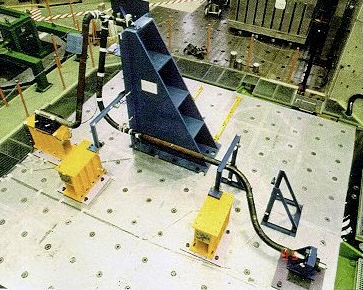
\includegraphics[width=4.8cm]{figures/intro-frags/ASG.jpg}
    \hspace{1cm}
    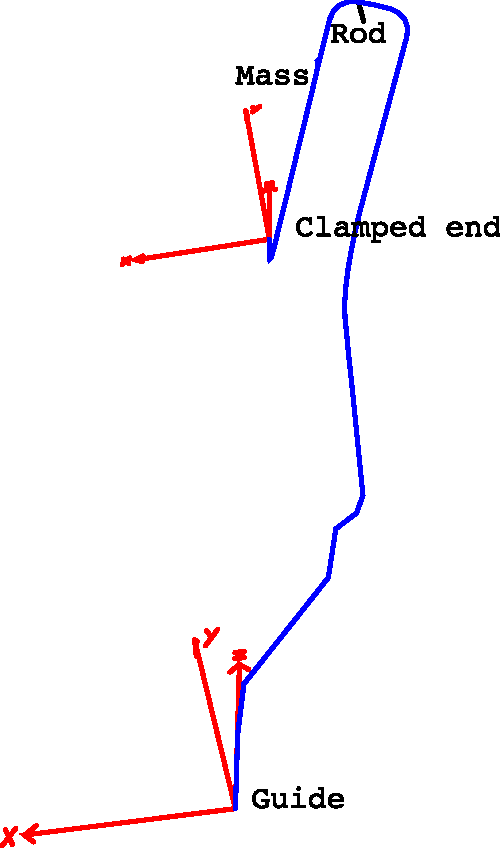
\includegraphics[width=2.3cm]{figures/intro-frags/ASG_FEM.pdf}
    \caption{(left) Overview of the piping system on the Azalee shaking table and (right) Mock-up FEM.}
    \label{lowdoe:fig:ASG}
\end{figure*}


\subsection{Benchmarking metrics}\label{lowdoe:sec:benchamrk}

In order to evaluate the effects that our planning of experiments method has over the fragility curve estimates, we consider four quantitative metrics described hereafter. Those are later implemented on the \emph{a posteriori} estimates conditional to two types of dataset: one derived from our planning of experiments methodology, and one without.
Considering a sample $(\mbf a, \mbf y)$, we denote
by $a \mapsto P_f^{|\mbf a, \mbf y}(a)$ the random process defined as the fragility curve conditionally to the sample. $P_f^{|\mbf a,\mbf y}(a)=\Phi((\rho\log a+\mu)/\sigma)$ inherits from the \emph{a posteriori} distribution of $\theta$.  
For each value $a$ the $r$-quantile of the random variable $P_f^{|\mbf a,\mbf y}(a)$ is denoted by $q_r^{|\mbf a,\mbf y}(a)$, and its median is denoted by $m^{|\mbf a,\mbf y}(a)$.  
Also, we take into account the reference fragility curve $a\mapsto P_f^{\mathrm{ref}}(a)$, evoked in \cref{lowdoe:sec:casestudy}; and we consider a bounded set $\cA=[0,A_{\max}]$ for the IM, the truncation is set to the maximal IM within the database of $10^4$ seismic signals we have at disposal for this work, as disclosed in \cref{lowdoe:sec:casestudy}. % generated from the stochastic simulator of~\cite{Rezaeian2010} and implemented in~\cite{Sainct2020}.
    We define:
    \begin{itemize}
        \item The square bias to the median: $\displaystyle{\cB^{|\mbf a,\mbf y} = \|m^{|\mbf a,\mbf y}- P_f^{\mathrm{ref}}\|^2_{L^2};\quad \text{where}\quad\|P\|^2_{L^2} = \frac{1}{A_{\max}}\int_{0}^{A_{\max}}P(a)^2 d a.}$
           % \begin{equation}
           %     \cB^{|\mbf a,\mbf y} = \|m^{|\mbf a,\mbf y}- P_f^{\mathrm{ref}}\|^2_{L^2};\quad \text{where}\quad\|P\|^2_{L^2} = \frac{1}{A_{\max}}\int_{0}^{A_{\max}}P(a)da.
           % \end{equation}
        \item The quadratic error: $\displaystyle{\cE^{|\mbf a,\mbf y} = \EE\left[\|P_f^{|\mbf a,\mbf y}-P_f^{\mathrm{ref}} \|^2_{L^2}|\mbf a,\mbf y\right].}$
            %\begin{equation}
            %    \cE^{|\mbf a,\mbf y} = \EE[\|P_f^{|\mbf a,\mbf y}-P_f^{\mathrm{ref}} \|^2_{L^2}|\mbf a,\mbf y].
            %\end{equation}
        \item The $1-r$-square credibility width: $\displaystyle{\cW^{|\mbf a,\mbf y} = \|q_{1-{r/2}}^{|\mbf a,\mbf y} - q_{{r/2}}^{|\mbf a,\mbf y}\|_{L^2}^2  .}$
            %\begin{equation}
            %    \cW^{|\mbf a,\mbf y} = \|q_{1-{r/2}}^{|\mbf a,\mbf y} - q_{{r/2}}^{|\mbf a,\mbf y}\|_{L^2}^2  .
            %\end{equation}
        \item The $1-r$-coverage probability: % zone's trustworthiness: 
        $\displaystyle{\cP^{|\mbf a,\mbf y} = \frac{1}{A_{\max}}\int_0^{A_{\max}}\indic_{P_f^{\mathrm{ref}}(a)\in \left[q_{1-{r/2}}^{|\mbf a,\mbf y}(a), q_{{r/2}}^{|\mbf a,\mbf y}(a) \right] } d a.}$
            %\begin{equation}
            %    \cT^{|\mbf a,\mbf y} = \frac{1}{A_{\max}}\int_0^{A_{\max}}\indic_{P_f^{\mathrm{ref}}(a)\in \left[q_{1-{r/2}}^{|\mbf a,\mbf y}(a), q_{{r/2}}^{|\mbf a,\mbf y}(a) \right] } da.
            %\end{equation}
    \end{itemize}
For the forthcoming implementation of these metrics, numerous \emph{a posteriori} samples of the process $P_f^{|\mbf a,\mbf y}$ are generated from their known distribution (see \cref{lowdoe:eq:posterior}) and serve the computation of the medians, quantiles and means through Monte-Carlo derivations. The integrals are approximated numerically from Simpsons' interpolation
{on sub-intervals of regular size  $0=A_0<\dots<A_p=A_{\rm max}$. In our computations, we use  $A_{\rm max}=55\,\mathrm{m/s^2}$, and $p=200$.}



\subsection{Numerical results}\label{lowdoe:sec:results}

%
\Cref{lowdoe:fig:examples} shows examples of fragility curve estimations based on different dataset sizes. 
%Both estimations differ only from their observation samples. 
The results presented in \cref{lowdoe:fig:examples}-(c) come from our planning-of-experiments (PE) methodology while the results presented in \namecrefs{lowdoe:fig:examples}~\ref{lowdoe:fig:examples}-(a) and~\ref{lowdoe:fig:examples}-(b) come from independent random samples, with IMs that have been drawn w.r.t. their original standard distribution or w.r.t. a uniform distribution. These qualitative results clearly illustrate the contribution of our methodology.




\begin{figure}[h]
    \centering%
    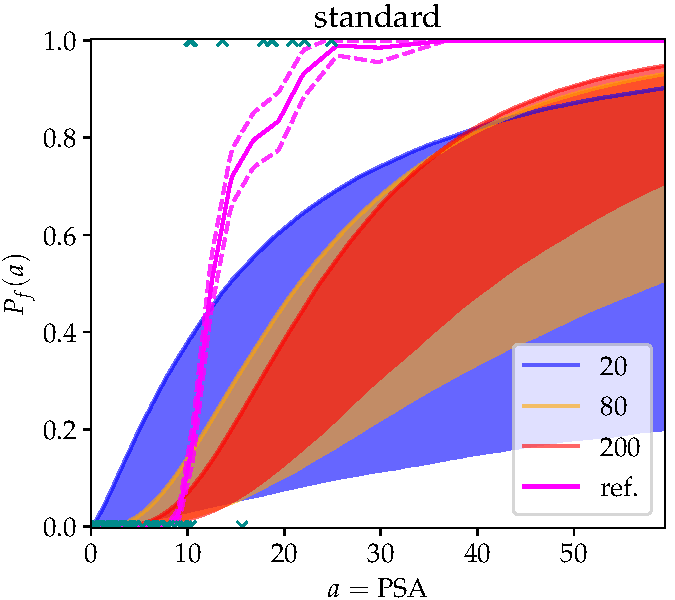
\includegraphics[width=5cm]{figures/low-doe/curves_standard.pdf}%
    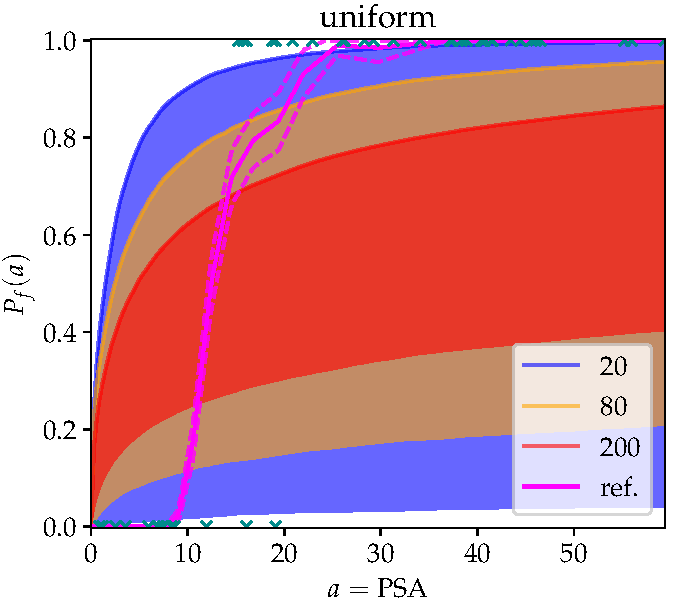
\includegraphics[width=5cm]{figures/low-doe/curves_unif.pdf}%
    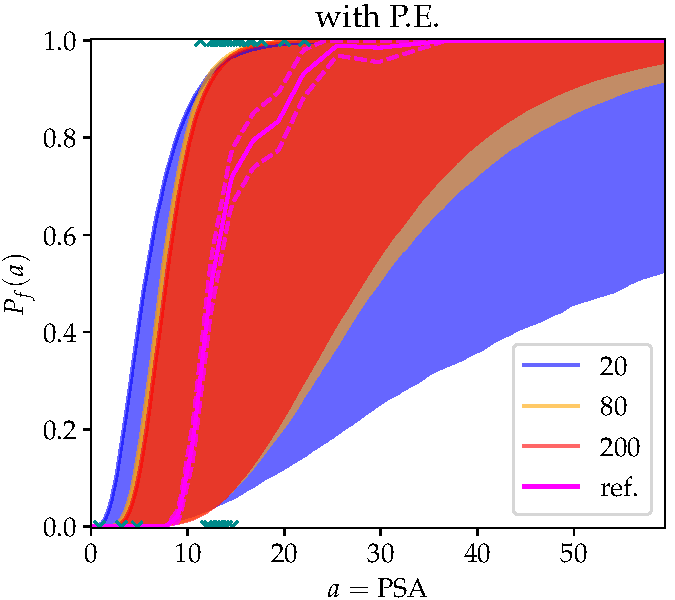
\includegraphics[width=5cm]{figures/low-doe/curves_PE.pdf}\\
    \hspace*{1.7em}{\hspace{\stretch{1}}(a)\hspace{\stretch{2}}(b)\hspace{\stretch{2}}(c)\hspace{\stretch{1}}\ }
    % \begin{tabular}{ccc}
    %    (a)  & (b) & (c) \\
    %      & 
    % \end{tabular}
    % \includegraphics[width=0.36\linewidth]{figures/low-doe/ASG_nlin_PSA_refMC/ex_stan_IC_ref.pdf}\hspace*{1em}%
    % \includegraphics[width=0.36\linewidth]{figures/low-doe/ASG_nlin_PSA_refMC/ex_PE_IC_ref.pdf}%    
    \caption{Examples of fragility curve estimations for different number of observations, with the PSA considered as IM. Are plotted the $95\%$ credibility interval for 3 datasets of respective sizes 20 (blue), 80 (orange), and 200 (red); the reference curve $P_f^{\mathrm{ref}}$ is drawn in magenta and is accompanied with the confidence interval of the procedure in dashed lines.
    The observations are chosen (a) w.r.t.{ }the standard distribution of the IM; 
    {or (b) w.r.t.{ }a uniform distribution on $[0,A_{\rm max}]$};
    or (c) using our planning of experiments method. The green crosses represent 50 pairs $(a_i,\indic_{y_i>C})$ drawn for each method.}
    \label{lowdoe:fig:examples}
\end{figure}


%Indeed, under a standardly drawn sample (understand here that the observed IM are independently sampled  w.r.t.{ }their original distribution), a fast convergence of the estimate is performed when the number of observation rises, with credibility intervals that get thinner accordingly.
%However, such strong convergence targets an incorrect value, that we suppose being due to the  bias of the linear model.

When samples are randomly drawn from the original IM distribution {or from a uniform distribution}, the results show a rapid convergence of the estimates ---in the sense that the associated credibility intervals decrease rapidly--- towards biased estimations of the fragility curves. Conversely, when the samples come from the PE methodology, the bias decreases but the convergence is slower.

These observations are confirmed on a larger scale by the results presented in \cref{lowdoe:fig:errors,lowdoe:fig:credibility}. 
These are issued from computations of the metrics $\cB^{|\mbf a,\mbf y}$, $\cE^{|\mbf a,\mbf y}$, $\cW^{|\mbf a,\mbf y}$ and $\cP^{|\mbf a,\mbf y}$ described in \cref{lowdoe:sec:benchamrk}, for various observation sets $(\mbf a,\mbf y)$. They compare the performances of our PE methodology with the two methods that are based on independently drawn observations: the one that involves  IM samples drawn from their standard distribution, and the one that involves IM samples drawn from a uniform distribution over the range $[0,A_{\rm max}]$.

\Cref{lowdoe:fig:errors} shows empirical comparisons of the bias and of the quadratic error between the method involving a design of experiments and without. These two results clearly illustrate that the PE approach outperforms the standard {and the uniform} approaches. Although the quadratic error is strongly related to the variance of the estimates it is significantly offset by the fact that the bias is smaller with the PE approach. Indeed, \cref{lowdoe:fig:credibility}-left illustrates that the $95\%$-square credibility width is smaller with the standard {and uniform} approaches than with the PE-based approach. This good result nevertheless masks a lack of robustness of the standard {or uniform}  approaches since the estimate turns out to be strongly biased, as shown in \cref{lowdoe:fig:credibility}-right. This figure shows indeed the coverage probability for the both methods, as a function of the dataset size. %It measures the average inclusion of the reference fragility curves to the \emph{a posteriori} credibility intervals.
It measures the average inclusion of reference fragility curves in posterior credibility intervals.


%Secondly, that last point is emphasized by what is shown in  Indeed, the standard method is there exposed to provide credibility intervals that get strongly thinner than the ones benefiting from P.E. 
%Yet, \cref{lowdoe:fig:credibility}-right unveils their lack of robustness under the first method. That last figure plots the coverage probability of both methods as a function of the dataset size. It measures the average belonging of the reference within the \emph{a posteriori} credibility intervals. The P.E. handles to avoid the trap of the model bias within the reliable credibility intervals it issues.





\begin{figure}[h!]
    \centering%
    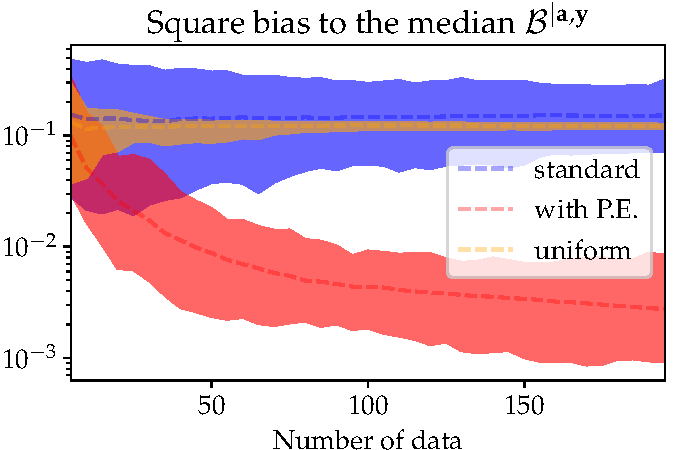
\includegraphics[width=5cm]{figures/low-doe/errB.pdf}%
    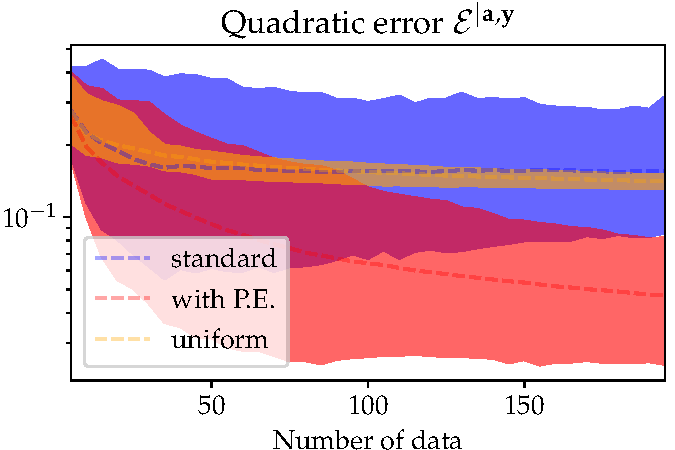
\includegraphics[width=5cm]{figures/low-doe/errE.pdf}%    
    \caption{Confidence intervals and means w.r.t.{ }the 
    $(\mbf a,\mbf y)$ for (left) the square bias to the median $\cB^{|\mbf a,\mbf y}$ and (right) the quadratic error $\cE^{|\mbf a,\mbf y}$; as a function of the number of observations. For each value of $k=5,10,\dots,200$, a number of $L=200$ dataset have been drawn following the standard distribution of the IM firstly (for the blue curves), {following a uniform distribution on $[0,A_{\rm max}]$ secondly (for the orange curves)}, and following the planning of experiments method thirdly (for the red curves). }
    \label{lowdoe:fig:errors}
\end{figure}


\begin{figure}[h!]
    \centering%
    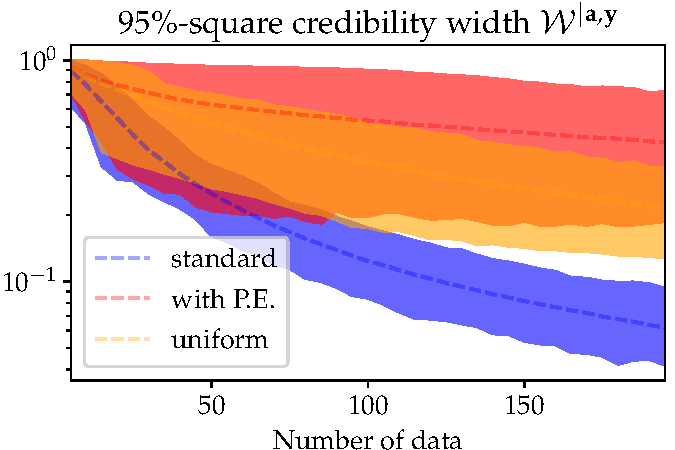
\includegraphics[width=5cm]{figures/low-doe/errW.pdf}%
    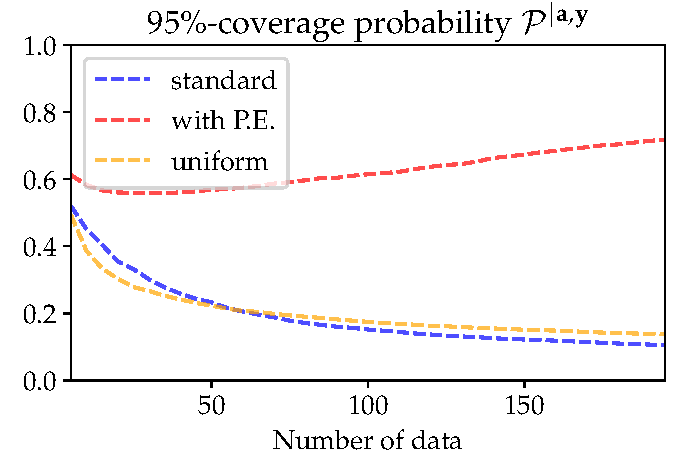
\includegraphics[width=5cm]{figures/low-doe/errP.pdf}%    
    \caption{(left) $95\%$-confidence intervals and means w.r.t.{ }$(\mbf a,\mbf y)$ for the $95\%$-square credibility width $\cW^{|\mbf a,\mbf y}$, as a function of the number of observations. (right) mean w.r.t.{ }$(\mbf a,\mbf y)$ for the $95\%$-coverage probability $\cP^{|\mbf a,\mbf y}$, as a function of the number of observations. For each value of $k=5,10,\dots,200$, $L=200$ datasets have been drawn following the standard distribution of the IM firstly (for the blue curves), {following a uniform distribution on $[0,A_{\rm max}]$ secondly (for the orange curves)}, and following the planning of experiments method thirdly (for the red curves).} %; the trustworthy of the credibi credibility zone is considered trustworthy if }
    \label{lowdoe:fig:credibility}
\end{figure}

\section{Discussion}\label{lowdoe:sec:discussion}

The results presented in the previous section clearly illustrate the superiority of the PE-based approach over the standard {and uniform} approaches. Similar results, not presented here for the sake of brevity, and obtained with the PGA as IM, as well as with other types of structures, also confirm these results.

The strength of the approach proposed in this work is its completely analytical nature, which avoids the use of MCMC methods for the \emph{a posteriori} estimation of fragility curves. To do this, however, it is necessary to assume that the logarithm of the EDP evolves linearly as a function of the logarithm of the IM.

So, to solve this problem, we are faced with a contradiction. In order to satisfy the linearity assumption, it is necessary, on the one hand, that the learning zone is local, that is to say restricted to the vicinity of the IMs for which the fragility curve evolves significantly from 0 to 1. On the other hand, \cref{lowdoe:eq:apostcf} shows that an empirical variance of the IMs that is too small is penalizing from the point of view of the variance of the estimation of the fragility curves. The variance of the latter is in fact inversely proportional to that of the IMs considered for learning.

As the numerical results show, the proposed learning method localizes the learning in the area of interest and significantly reduces the model bias. As a result, this is accompanied by a slight reduction in the size of the credibility interval with the number of training data.

This therefore suggests that the proposed method is effective for samples
with limited size (for instance, given the results presented in \cref{lowdoe:sec:results}, an appropriate limit could be a sample size smaller than 100 for the case study treated in this appendix). Beyond that, given the cost associated with each training data, it seems preferable to move towards less constrained and more sophisticated methods.

\section{Conclusion}\label{lowdoe:sec:conclusion}

Assessing the seismic fragility of structures and components when few data are available is a challenging task and the Bayesian framework is known to be effective for these types of problems.

In this work we proposed an efficient Bayesian methodology whose strength lies in its fully analytical nature, which avoids the use of MCMC methods for the \emph{a posteriori} estimation of fragility curves.
The effectiveness of the method comes from the assumption of linearity between the logarithm of the EDP and that of the IM of interest. As this hypothesis implies a model bias in most practical cases, we proposed a strategy in order to minimize this bias, by concentrating the learning in the vicinity of the IMs for which the fragility curve evolves significantly from 0 to 1.

The numerical results clearly illustrate the superiority of the proposed approach over an approach without a learning strategy. 
They emphasize the robustness of a design of experiments which is based on a sensitivity analysis of the posterior distribution.
 Such construction is not limited to the modeling we derive in this work in particular, and could still be adapted to another to increase its learning abilities. 
They also suggest that the proposed method is effective for a limited sample size (about 100 in our settings). Beyond that, given the cost associated with each training data, it seems preferable to move towards less constrained and more sophisticated methods, in order to more effectively minimize both the biases and the variance of the estimates.

For practitioners, this method therefore constitutes a rapid and robust tool for first estimates of fragility curves in a context where the datasets are of limited size.

%As the design of experiment 



% \appendix

\section{Details regarding the construction of $\mbf z$}\label{lowdoe:app:sec:DiagUa}

%\subsection{Definition}
%\paragraph{Diagonalization of $U_{\mbf a}$} 

%Now consider the pair $\xi=(\mu,\sigma)$, for it can be build a likelihood as
Conditionally to $(\mbf a, \theta)$, we derive the distribution of $\hatmbf y-\rho_k\hatmbf a$: 
    \begin{equation}\label{lowdoe:eq:likelihood2}
        \hatmbf y - \rho_k\hatmbf a|\mbf a, \theta \sim\cN(\mu \mbf 1, \sigma^2 U_{\mbf a})  , \quad\text{with}\quad U_{\mbf a} = I - \frac{\hatmbf a(\frac{1}{2}\hatmbf a - \overline{\hatmbf a})^{\top}  }{k\Var_k\hatmbf a} - \frac{(\frac{1}{2}\hatmbf a - \overline{\hatmbf a}) \hatmbf a^{\top}  }{k\Var_k\hatmbf a} ,\quad \overline{\hatmbf a} = \frac{1}{k}\sum_{i=1}^k \log a_i,
        %\\
        % &\ell_k(\mbf z |\mbf a,\xi) = \prod_{i=1}^k\frac{1}{\sqrt{2\pi}\sigma}\exp\left(-\frac{(z_i - \mu U_{\mbf a,i}^{-1/2})^2}{2\sigma^2}  \right)
    \end{equation}
where $\mbf 1$ denotes the vector of $\RR^k$ which contains only ones. %, and the matrix $U_{\mbf a}$ is given by
% \begin{equation}
%     U_{\mbf a} = I - \frac{\hatmbf a(\frac{1}{2}\hatmbf a - \overline{\hatmbf a})^{\top}  }{k\Var_k\hatmbf a} - \frac{(\frac{1}{2}\hatmbf a - \overline{\hatmbf a}) \hatmbf a^{\top}  }{k\Var_k\hatmbf a}\ ;\quad \overline{\hatmbf a} = \frac{1}{k}\sum_{i=1}^k \log a_i.
% \end{equation}
Below is suggested a diagonalization of the matrix $U_{\mbf a}$: we define $P_{\mbf a}$ such that $P_{\mbf a}^{\top}P_{\mbf a}=I$ and $P_{\mbf a}^{\top}U_{\mbf a}P_{\mbf a}$ is a diagonal matrix. To define $\mbf z$, we denote by $\tilde P_{\mbf a}$ the matrix in $\RR^{k\times(k-1)}$ composed by the $k-1$ first columns of $P_{\mbf a}$. {In what follows, we assume that $k>2$ and that the coordinates of $\mbf a$ are not all identical.} \\


The matrix $U_{\mbf a}$ takes the form of $I-uv^{\top}-vu^{\top}$ for some vectors $u$ and $v$ of $\RR^k$, which are linearly independent. It is clear that the diagonalization of $U_{\mbf a}$ is linked with the one of $V=uv^{\top}+vu^{\top}$.

First of all notice that $v^\perp$ and $u^\perp$ are two different hyperplanes because of the linear independence of $u$ and $v$. That makes $u^\perp\cap v^\perp$ a subspace of dimension $k-2$. %; and $u^\perp\prive\RR v$, $v^\perp\prive\RR u$ two non empty sets.
Therefore, as one would notice that $u^\perp\cap v^\perp\subset\Kernel V$ and $\Image V\subset\Span(u,v)$, the converse inclusions stand.

This way, while $0$ is the first eigenvalue of $V$ with rank $k-2$, an other eigenvalue $r$ must admit eigenvectors in $\Span(u,v)$, which should make the system
    \begin{equation}\label{lowdoe:app:eq:systemr}
        \left\{\begin{array}{rl}
             r\gamma &= \gamma v^{\top}u+\delta v^{\top}v  \\
             r\delta &= \gamma u^{\top}u + \delta u^{\top}v 
        \end{array}  \right.
    \end{equation}
admitting an infinity of solutions w.r.t.{ }$(\gamma,\delta)$. Equivalently, its determinant must be null which lead to the two solutions 
    \begin{equation}
        r = v^{\top}u \pm \|v\|\|u\|.
    \end{equation}
As $u$ and $v$ are linearly independent, the equation above defines two different eigenvalues $r_+$ and $r_-$, both of rank $1$.
Let $r$ be one of those, a resolution of the equation system~(\ref{lowdoe:app:eq:systemr}) gives that the eigenspace associated with $r$ is $\Span(v^{\top}vu+(r-v^{\top}u)v)$.\\

Coming back to $U_{\mbf a}$, the arguments above show that the eigenvalues of $U_{\mbf a}$ are $1$, $1-r_-$ and $1-r_+$ with respective ranks $k-2$, $1$ and $1$, and with:
\begin{equation}
    r_+ = 1 \ ,\quad r_- = \frac{- k\overline{\hatmbf a}^2}{\|\hatmbf a-\overline{\hatmbf a} \|^2},
\end{equation}
because 
\begin{equation}
    \|\hatmbf a\|^2\|\frac{1}{2}\hatmbf a - \overline{\hatmbf a} \|^2  = \sum_{i=1}^k\hat a_i^2
    \left(\frac{1}{4}\sum_{i=1}^k\hat a_i^2 + \left(\sum_{i=1}^k\hat a_i^2\right)\frac{1}{k}\left(\sum_{i=1}^k\hat a_i\right)^2 - \left(\sum_{i=1}^k\hat a_i^2\right)\frac{1}{k}\left(\sum_{i=1}^k\hat a_i \right)^2 \right)
        = \frac{1}{4}\left(\sum_{i=1}^k\hat a_i^2\right)^2. % \\
   % \mbox{and}\quad 
\end{equation}

Now, let us choose $w_1,\dots,w_{k-2}$ an orthonormal basis of $\hatmbf a^\perp\cap(\frac{1}{2}\hatmbf a-\overline{\hatmbf a})^\perp$. Let us define 
\begin{equation}\label{lowdoe:eq:wk-1.wk}
    w_{k-1} = \frac{1}{\sqrt k}\mbf 1 ,\quad w_{k} = \frac{\hatmbf a - \overline{\hatmbf a}}{\|\hatmbf a-\overline{\hatmbf a}\|}.
\end{equation}
% \begin{align}
%     w_{k-1} &= \frac{1}{\sqrt k}\mbf 1 \\ %\frac{\overline{\hatmbf a}\mbf 1}{\frac{1}{2}\hatmbf a^{\top}\hatmbf a} \\
%     w_{k} &= \frac{\hatmbf a - \overline{\hatmbf a}}{\|\hatmbf a-\overline{\hatmbf a}\|}.
% \end{align}
We remind $\mbf 1$ is the vector whose coordinates are ones. Therefore, denoting $P_{\mbf a}$ the matrix whose columns are the $w_i$, $i=1,\dots,k$; it comes $P_{\mbf a}^{\top}P_{\mbf a}=I$ and
    \begin{equation}
        P^{\top}_{\mbf a}U_{\mbf a}P_{\mbf a} = \diag\left(1,\dots,1,\frac{\hatmbf a^{\top}\hatmbf a}{\|\hatmbf a-\overline{\hatmbf a}\|^2}, 0\right).
    \end{equation}

% {The complete definition of $P_{\mbf a}$ depends on the chosen orthonormal basis $w_1,\dots,w_{k-2}$ of $\hatmbf a^\perp\cap(\frac{1}{2}\hatmbf a^\perp-\overline{\hatmbf a})$.
% In practice, we proceed as follows to construct them: from $w_{k-1}=(w_{k-1}^{(j)})_{j=1}^k$ and $w_k=(w_k^{(j)})_{j=1}^k$ as defined in equation (\cref{{lowdoe:eq:wk-1,wk}), we denote by $\tilde w_i=(\tilde w_i^{(j)})_{j=1}^k$ the vector of $\RR^k$ such that
% \begin{align}
%     (\tilde w^{(0)}_i,\,\tilde w_i^{(i)},\,\tilde w^{(i+1)}_i) &= (w^{(0)}_{k-1},\, w_{k-1}^{(i)},\,w^{(i+1)}_{k-1})\wedge (w^{(0)}_k,\,w_k^{(i)},\,w^{(i+1)}_k)\\ &= (w^{(i)}_{k-1}w^{(i+1)}_{k}-w^{(i)}_{k}w^{(i+1)}_{k-1},\, w^{(i+1)}_{k}w^{(0)}_{k-1}-w^{(i+1)}_{k-1}w^{(0)}_{k},\, w^{(0)}_{k-1}w_{k}^{(i)}-w^{(0)}_{k}w_{k-1}^{(i)}),\nonumber
% \end{align}
% and $\tilde w_i^{(j)}=0$ for any $j\not\in\{0,i,i+1\}$. That ensures the $\tilde w_i$, $i=1,\dots,k-2$ to form a basis of $\Span(w_{k-1},w_k)^\perp=\hatmbf a^\perp\cap(\frac{1}{2}\hatmbf a^\perp-\overline{\hatmbf a})$. Then, the orthonormal basis $w_1,\dots,w_{k-2}$ results from the Graam-Schmit process applied on $\tilde w_1,\dots\tilde w_{k-2}$.
% }


{The complete definition of $P_{\mbf a}$ depends on the chosen orthonormal basis $w_1,\dots,w_{k-2}$ of $\hatmbf a^\perp\cap(\frac{1}{2}\hatmbf a-\overline{\hatmbf a})^\perp$.
In practice, we proceed as follows to construct it, starting from $w_{k-1}=(w_{k-1}^{(j)})_{j=1}^k$ and $w_k=(w_k^{(j)})_{j=1}^k$ as defined in \cref{lowdoe:eq:wk-1.wk}. 
We denote by $e_i$ the canonical vectors of $\RR^k$ (the $j$th coordinate of $e_i$ is equal to $0$ iff $j\ne i$). As the coordinates of $\mbf a$ are not all the sames, there exist $j,p$ such that $w_{k}^{(j)}\ne w_{k}^{(p)}$ (in practice, we select the minimal $j$ and the minimal $p$ such that this property is verified). Thus, we can show that the vectors $w_k,w_{k-1},(e_i)_{i\ne j,p}$ form a basis of $\RR^k$ by computing their determinant:
    \begin{equation}
        \det(w_k,w_{k-1},(e_i)_{i\ne j,p}) = w_k^{(j)}w_{k-1}^{(p)}(-1)^{j+p+1} - w_{k-1}^{(j)}w_k^{(p)}(-1)^{j+p+1}\ne 0,
    \end{equation}
%with $\varepsilon$ being the determinent of the family $(e_i)_{i\ne j,p}$ after removing their $i$th and their $p$th row, so that $\varepsilon = 1$.
as $w_{k-1}^{(j)}=w_{k-1}^{(p)}$.
Eventually, the family of the $w_i,\,i=1,\dots k$ is the result of the Gram-Schmidt process applied to $u_k,\dots,u_1=w_k,w_{k-1},(e_i)_{i\ne j,p}$: 
    \begin{equation}
        w_{k-i} = \frac{\tilde w_{k-i}}{\|\tilde w_{k-i}\|},\qquad \tilde w_{k-i} = u_{k-i} - \sum_{j<i} w_{k-j}^{\top}u_{k-i}\cdot w_{k-j}, 
    \end{equation}
%with $\langle\cdot,\cdot\rangle$ denoting the usual scalar product in $\RR^k$. 
Note that this process leaves the expressions of $w_k$ and $w_{k-1}$ unchanged. The family $w_1,\dots,w_{k-2}$ thus forms a basis of $\Span(w_k,w_{k-1})^\perp=\hatmbf a^\perp\cap(\frac{1}{2}\hatmbf a-\overline{\hatmbf a})^\perp$.

We invite the reader to notice that in any way, the construction of those $k-2$ first columns of $P_{\mbf a}$ has no influence on the resulting posterior distribution of interest (given by \cref{lowdoe:eq:posterior}). Indeed, that latter only involves the expressions of $z_{k-1}$ and of $\sum_{i=1}^{k-2}z_i^2$. Concerning the first one, it is equal to $w_{k-1}^{\top}(\hatmbf y-\rho_k\hatmbf a)$, and concerning the second one, it is equal to:
    \begin{align*}
            \sum_{i=1}^{k-2}z_i^2=\sum_{i=1}^{k-2}|w_i^{\top}(\hatmbf y-\rho_k\hatmbf a)|^2&=\sum_{i=1}^{k}|w_i^{\top}(\hatmbf y-\rho_k\hatmbf a)|^2-|w_{k-1}^{\top}(\hatmbf y-\rho_k\hatmbf a )|^2-|w_k^{\top}(\hatmbf y-\rho_k\hatmbf a )|^2\\
                &=\|\hatmbf y-\rho_k\hatmbf a\|^2-|w_{k-1}^{\top}(\hatmbf y-\rho_k\hatmbf a )|^2-|w_k^{\top}(\hatmbf y-\rho_k\hatmbf a )|^2.
        \end{align*}
    }


\newpage
\thispagestyle{empty}

